\chapter{Single Input Single Output Line Of Sight Channel}

this is the simplest way to transmit a signal wirelessly, by using one antenna at both \Tx and \Rx. but this simplicity comes with it's costs.

\section{Antennas position}
for this system we use single antenna at the center of the \Tx and \Rx , which is (0,0,0) for the both proportional to their centers.\\
\Tx single input position $\to$ txsipos = (0,0,0)\\
\Rx single input position $\to$ rxsipos = (0,0,0)\\

\section{Scattering channel matrix}
\subsection{Scattering model}
is a model designed to describe the scattering of a radio waves in complex environments
\subsection{Scatteringchanmtx}
it's a function that generates a matrix that describes the wireless channel by based on the scattering model, by knowing:
\begin{enumerate}
	\item \Tx antenna array
	\item \Rx antenna array
	\item \Tx angle
	\item \Rx angle
	\item channel gain (gain = 1)
\end{enumerate}
\section{Eb/No}
it's the power of a single bit (Eb) divided by the spectral noise power density (No)\\
and it equals
$$
\frac{\text{Eb}}{\text{No}} = \text{SNR} \times \frac{\text{B}}{\text{R}_\text{b}}
$$
in our case we will use 11 different values for it to see the the effects on the communication system for different Eb/No values.

\section{Bit Error Rate (BER)}
it is the number of bit errors divided by the total number of transmitted bits over a given time interval.

in this project, we will calculate it by an assigned function called 'helpMIMOBER' which takes the scattering channel matrix, the original bit sequence (x) and Eb/No to calculate the BER.

in our case we want to monitor the relationship between Eb/No and BER in a SISO LOS channel so will use the 11 values of Eb/No and calculate the BER for each one using helpMIMOBER function.
\section{Plotting}
as we can see in Figure[\ref{fig:sisober}], the BER decreases as we increase the Eb/No.

and it's pretty striate forward, as long as we increase the ratio of the bit power over the noise spectral power, the probability of bit error decreases.

\begin{figure}[!h]
	\centering
	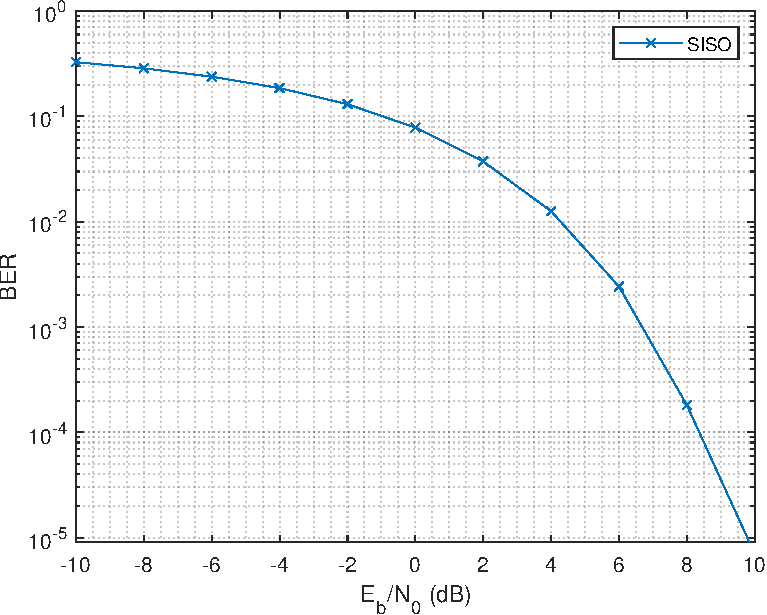
\includegraphics[width=1\linewidth]{figures/SISO_BER}
	\caption{SISO BER for each Eb/No}
	\label{fig:sisober}
\end{figure}



\newgeometry{margin=0pt}
\newpage
\vfill
\begin{figure}
	\centering
	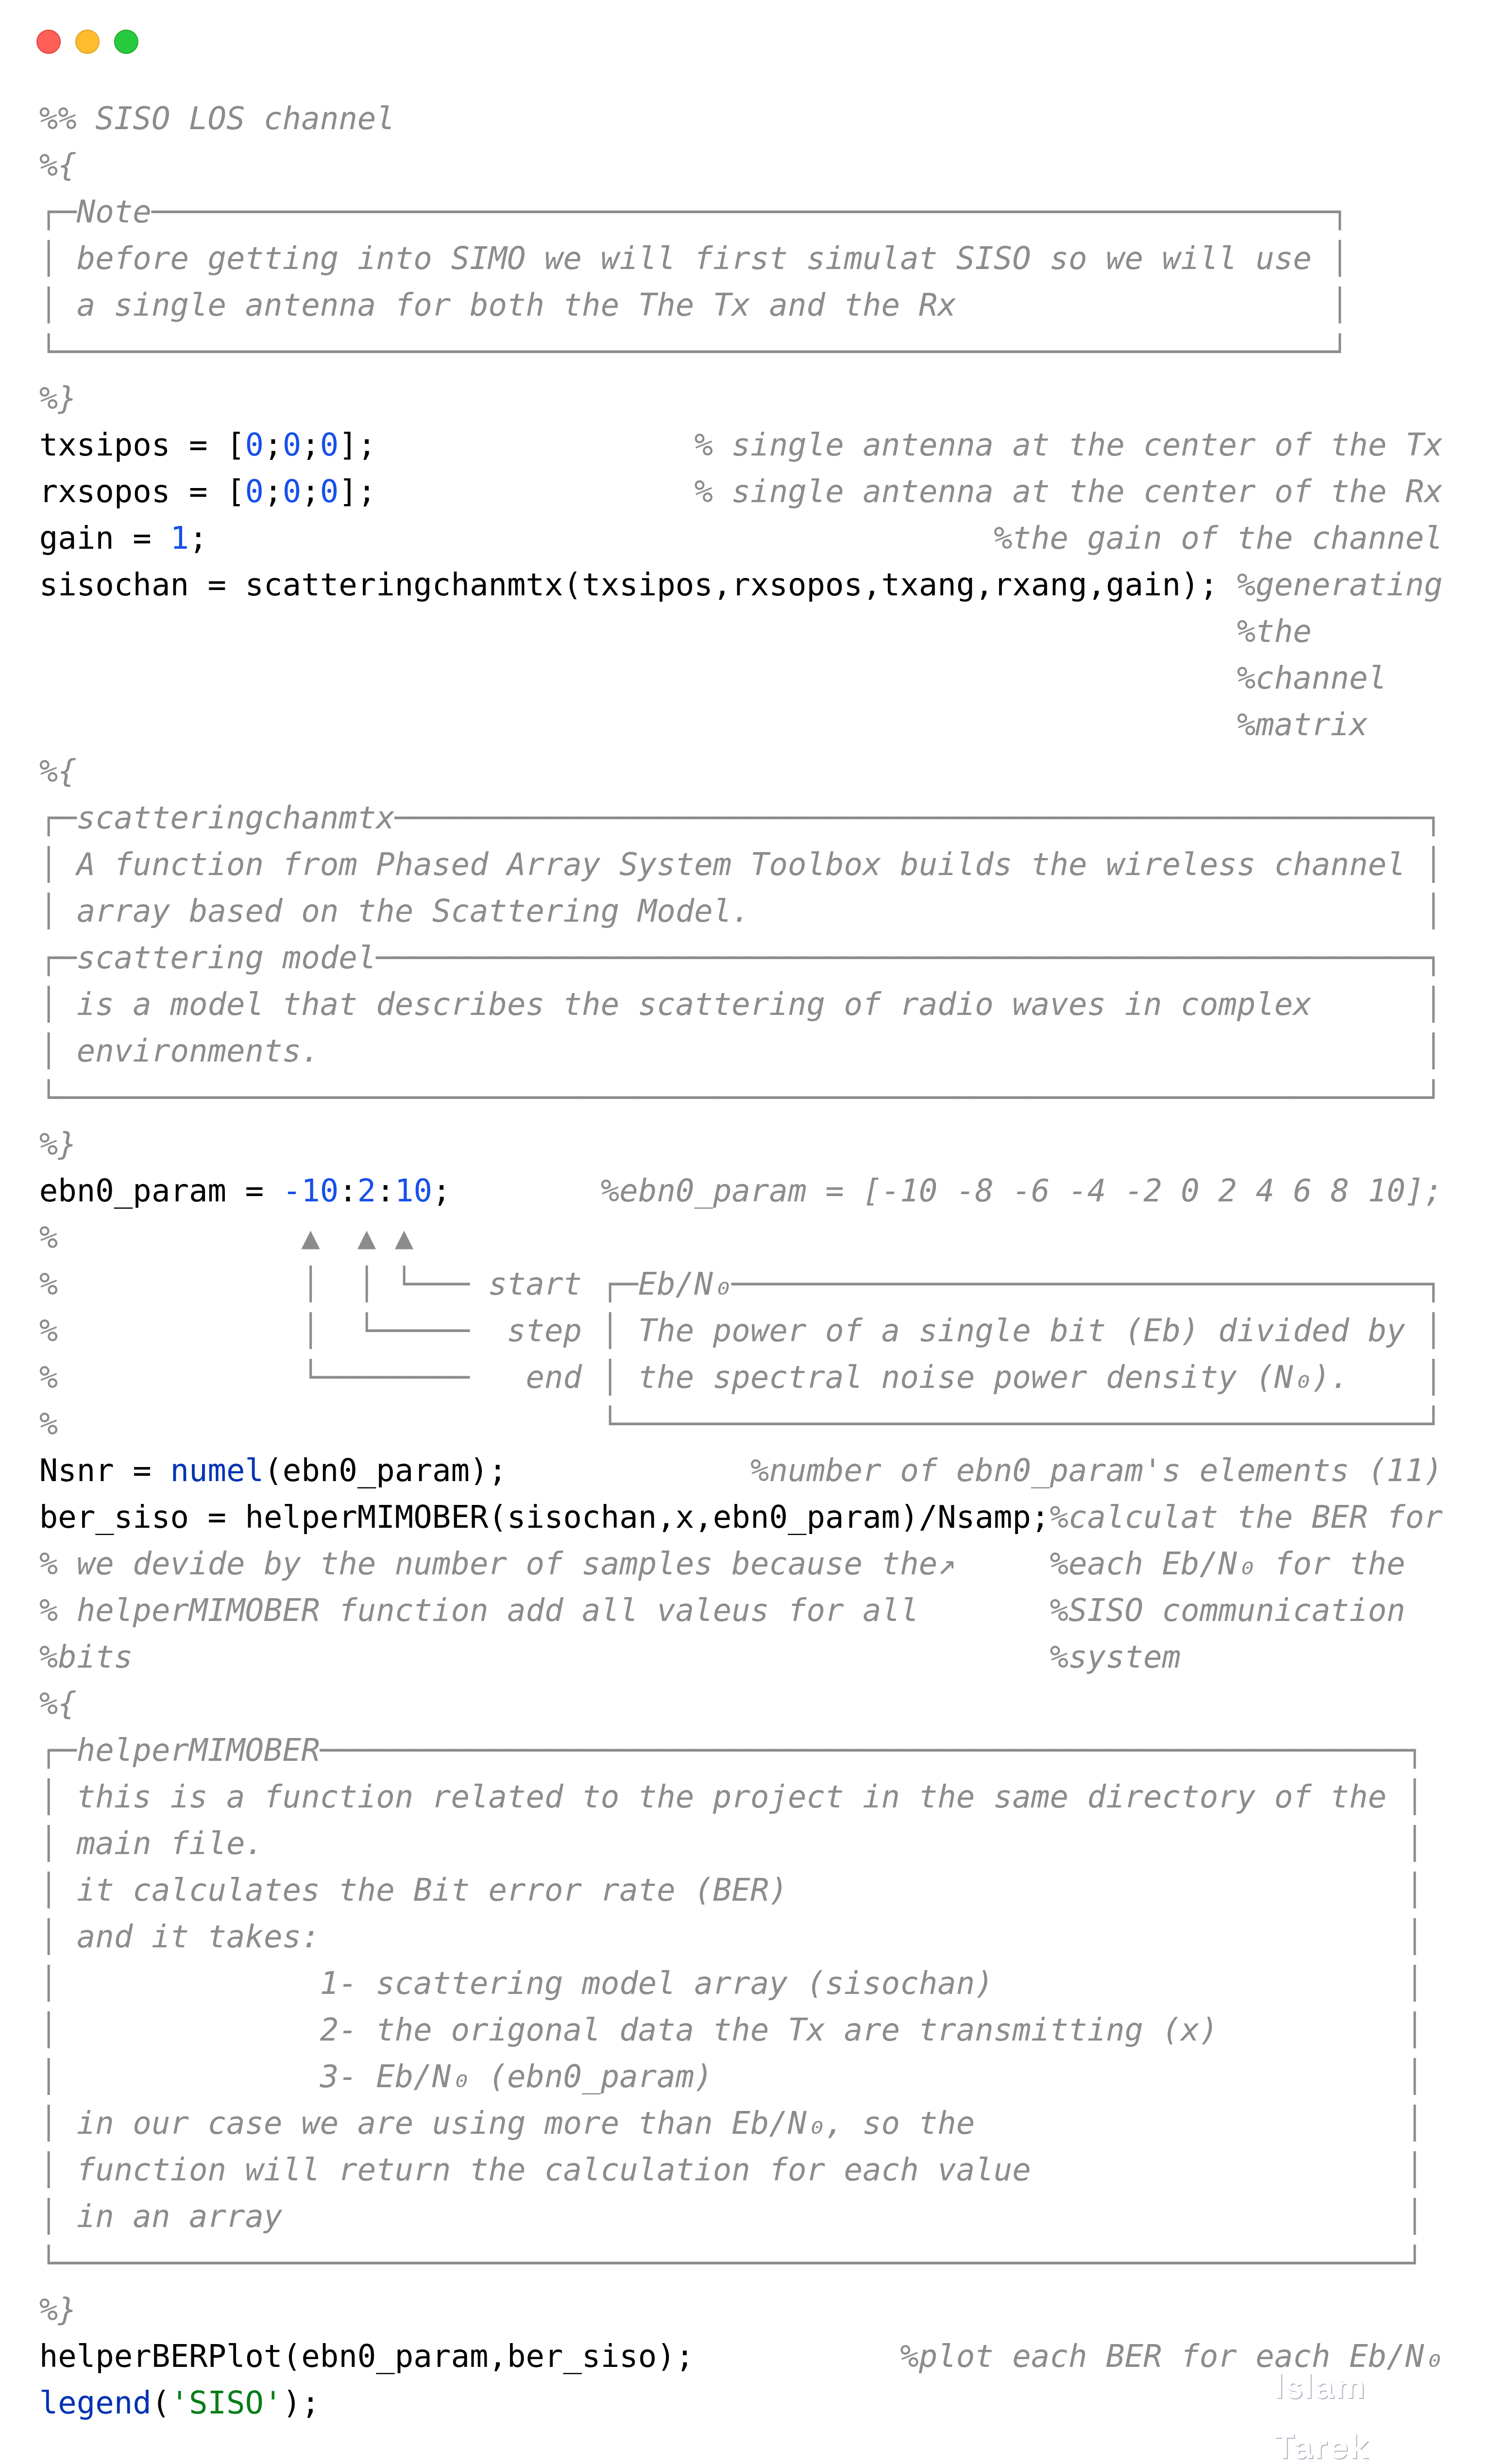
\includegraphics[width=0.8\linewidth]{figures/code2}
\end{figure}
\vfill
\restoregeometry